\subsection{Model}
The following model concerns the most characterizing features of the system. The model is intended as a static analysis, therefore it does not consider time or state transitions, but only invariant properties of the described world.
We avoided to burden the model with trivial and non-significant details.

\verbatiminput{alloy.als}

\subsection{Alloy result}
	The model is consistent: see Figure 4.
	\begin{figure}
		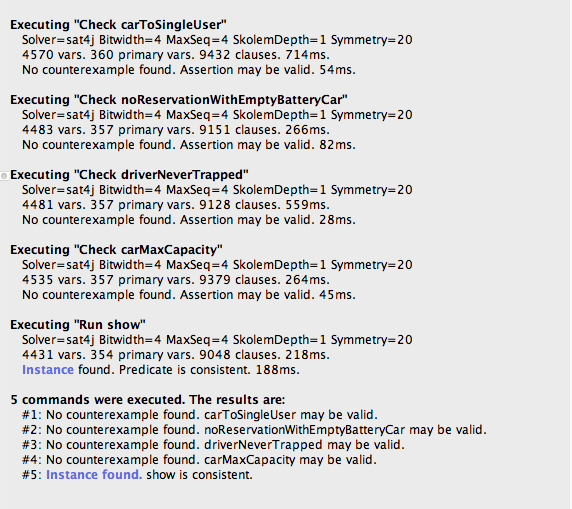
\includegraphics[width=\textwidth]{img/alloy_output.png}
		\caption{Result of the model analysis.}
		\label{figure 1}
	\end{figure}

	\begin{landscape}
		\subsection{Metamodel}
		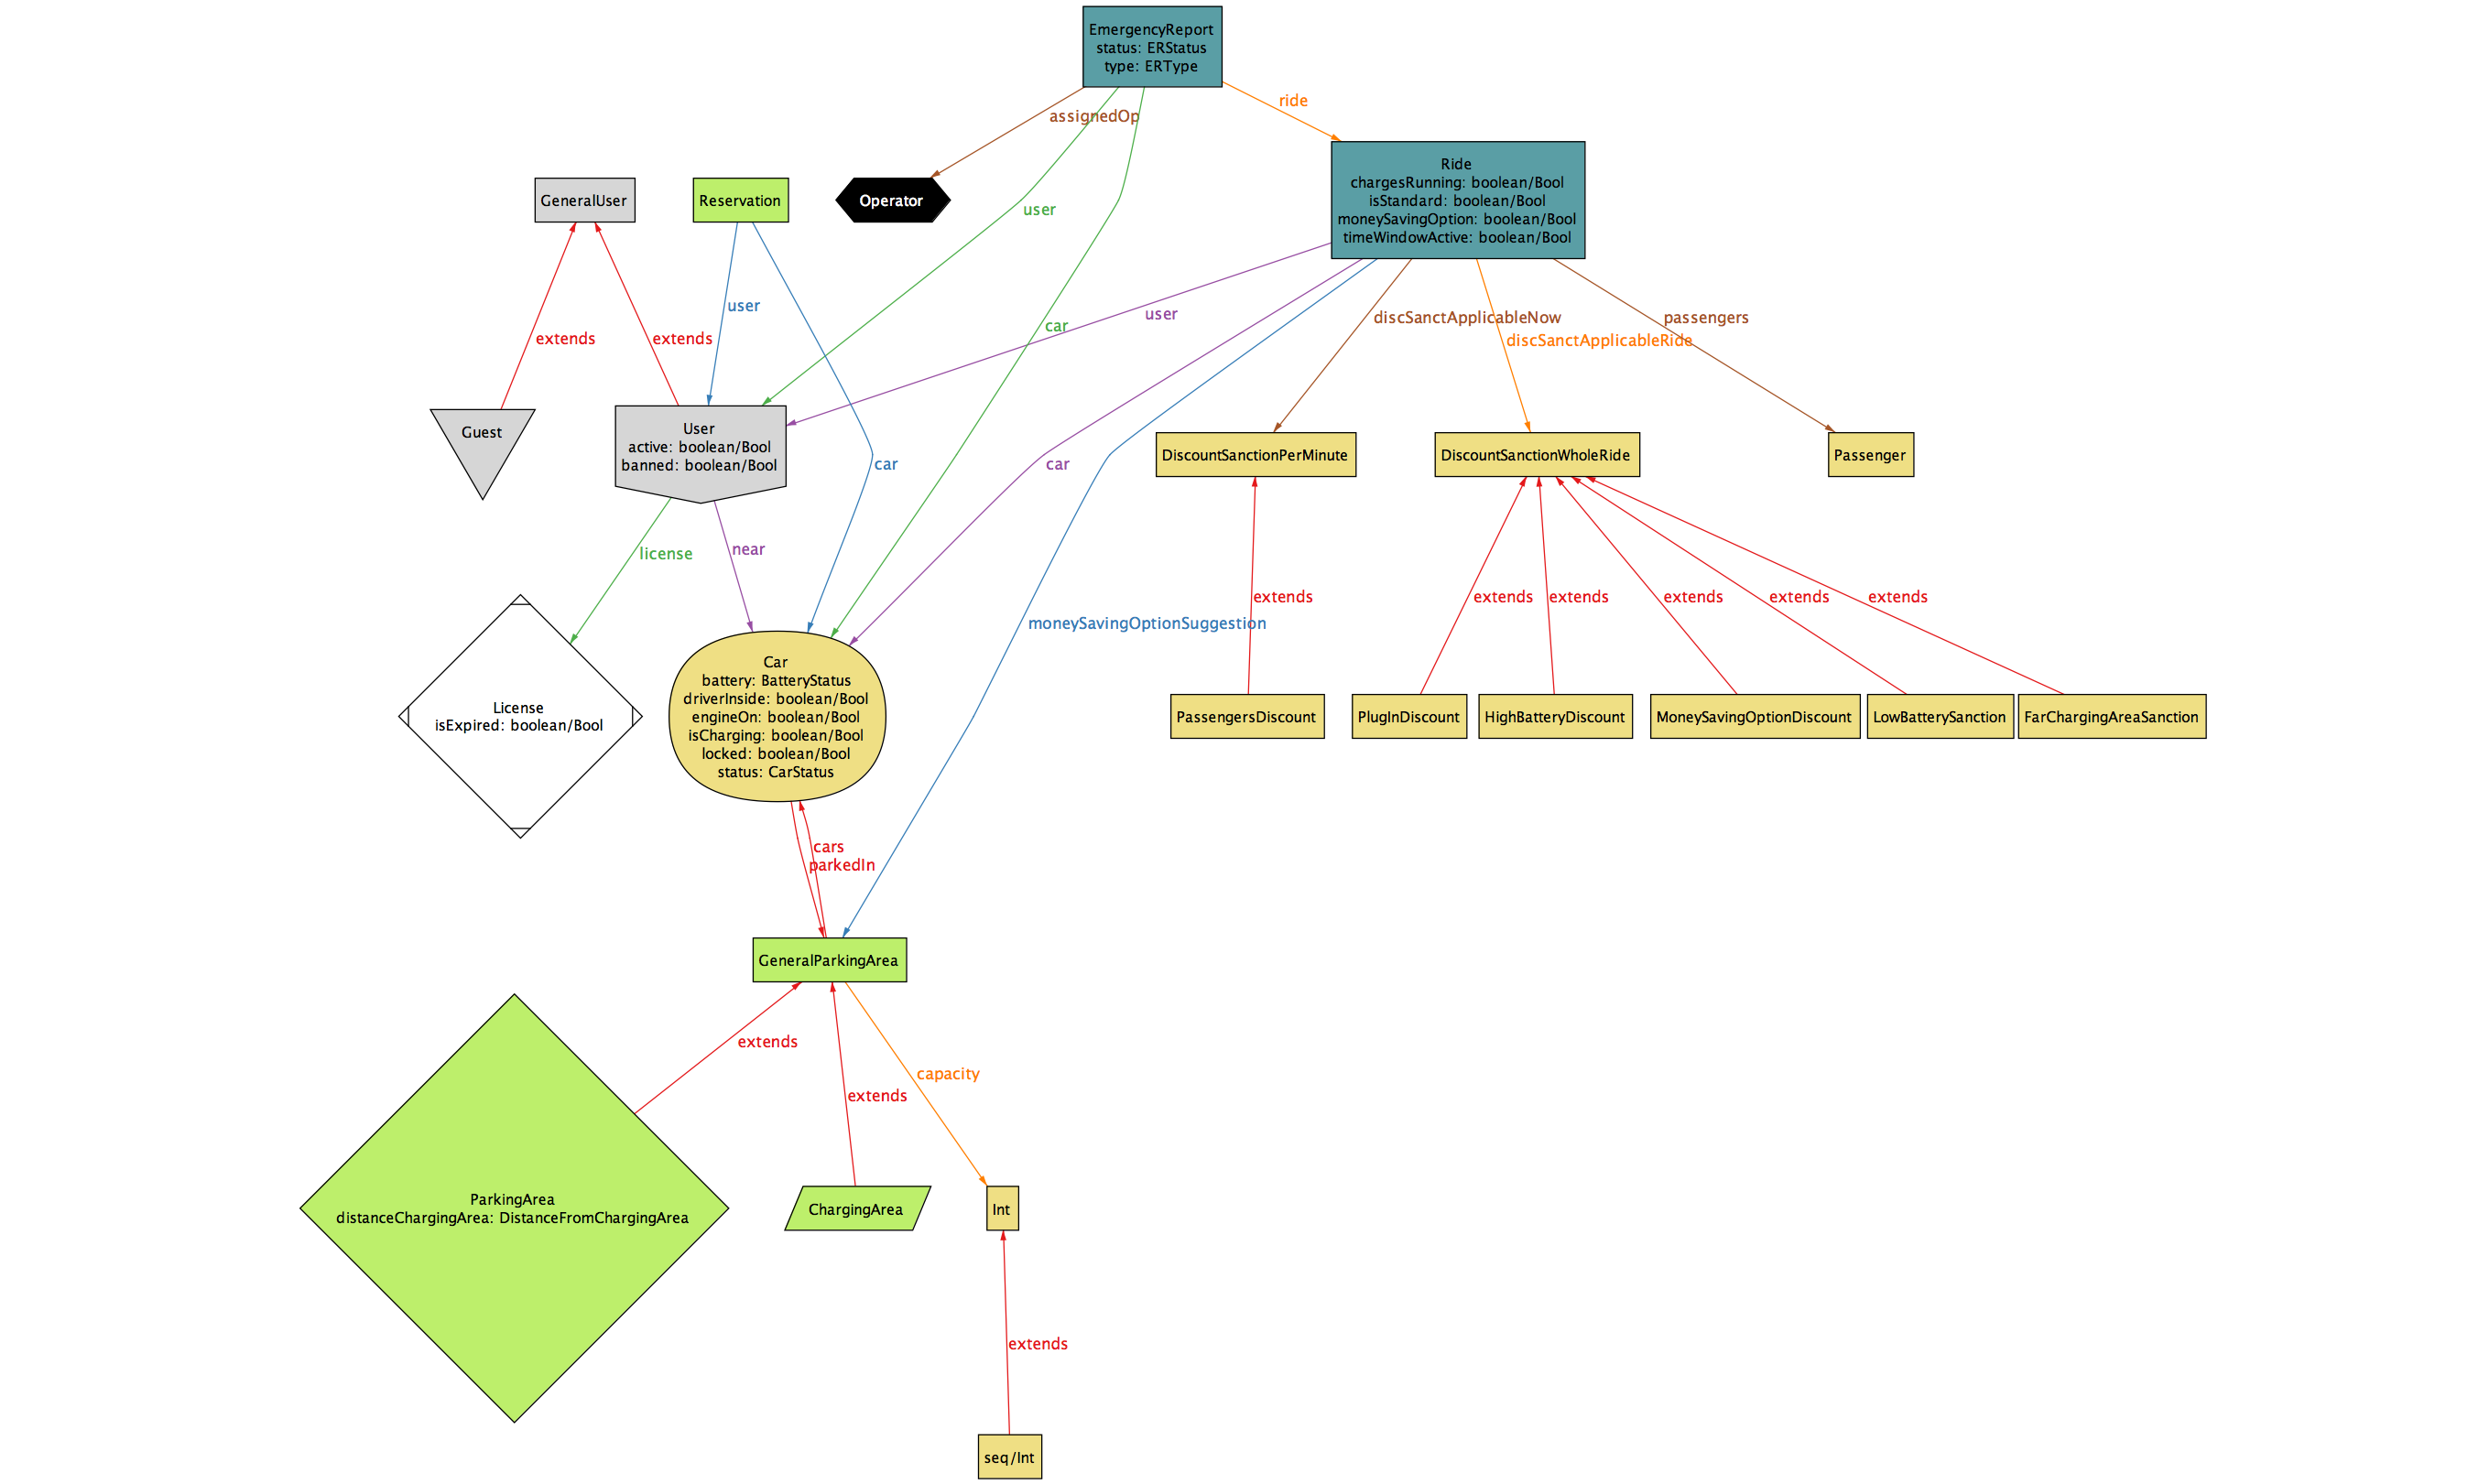
\includegraphics[width=1.5\textwidth, center]{img/metamodel.png}
	\end{landscape}

	\begin{landscape}
	
	\subsection{Worlds generated}
	
		\subsubsection{General world}
			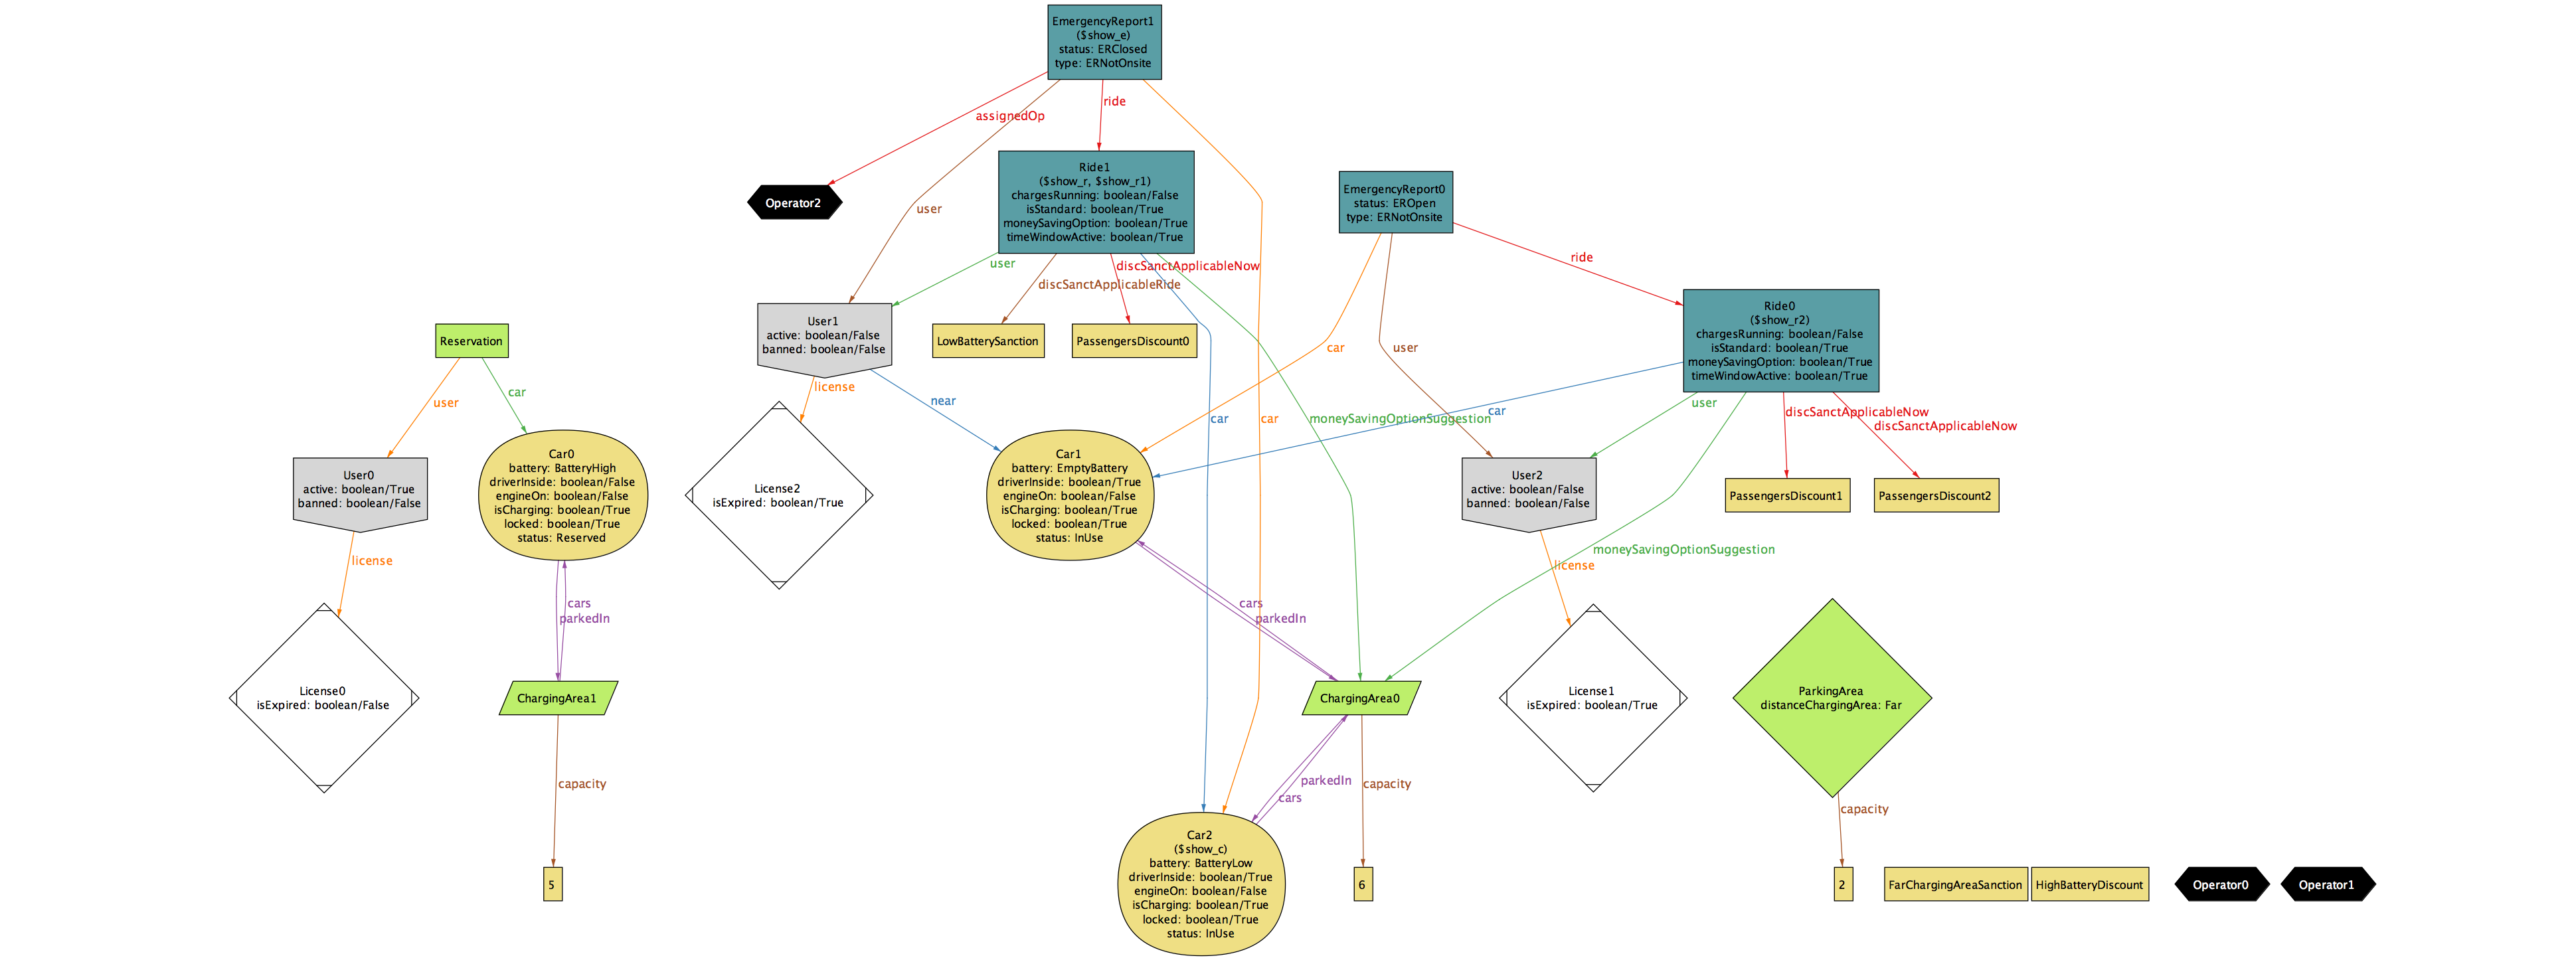
\includegraphics[height=\textheight, center]{img/world1.png}
	
		\subsubsection{Ride-reservation projection}
			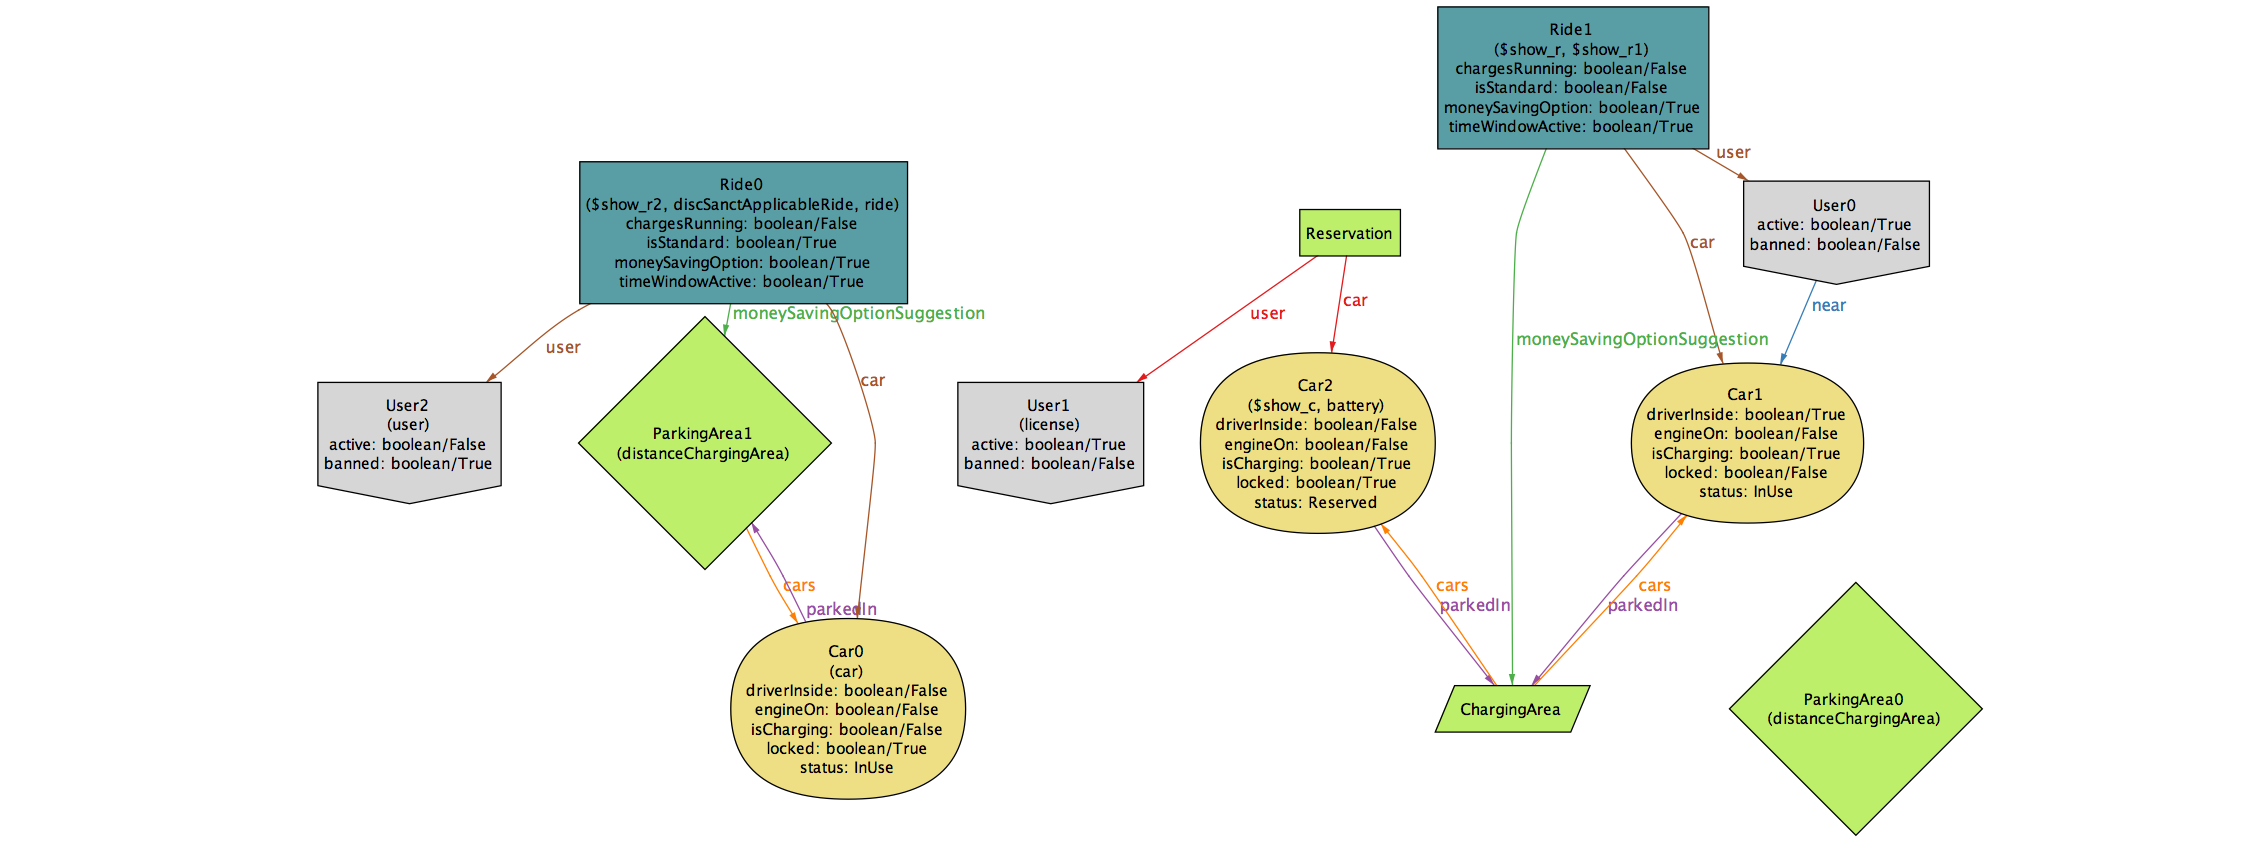
\includegraphics[width=2\textwidth, center]{img/rides_reservations.png}
	
		\subsubsection{User licenses projection}
			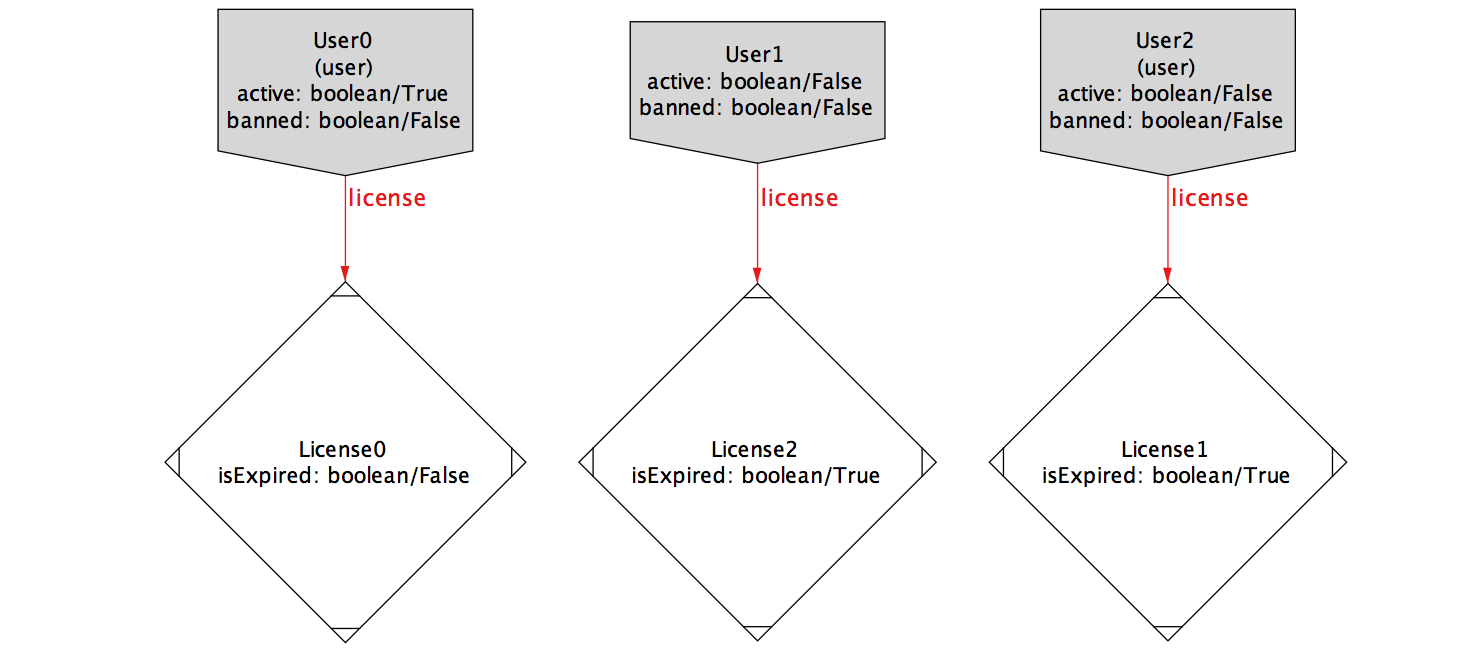
\includegraphics[width=2\textwidth, center]{img/user_licenses.png}
		
		\subsubsection{Emergency report projection}
			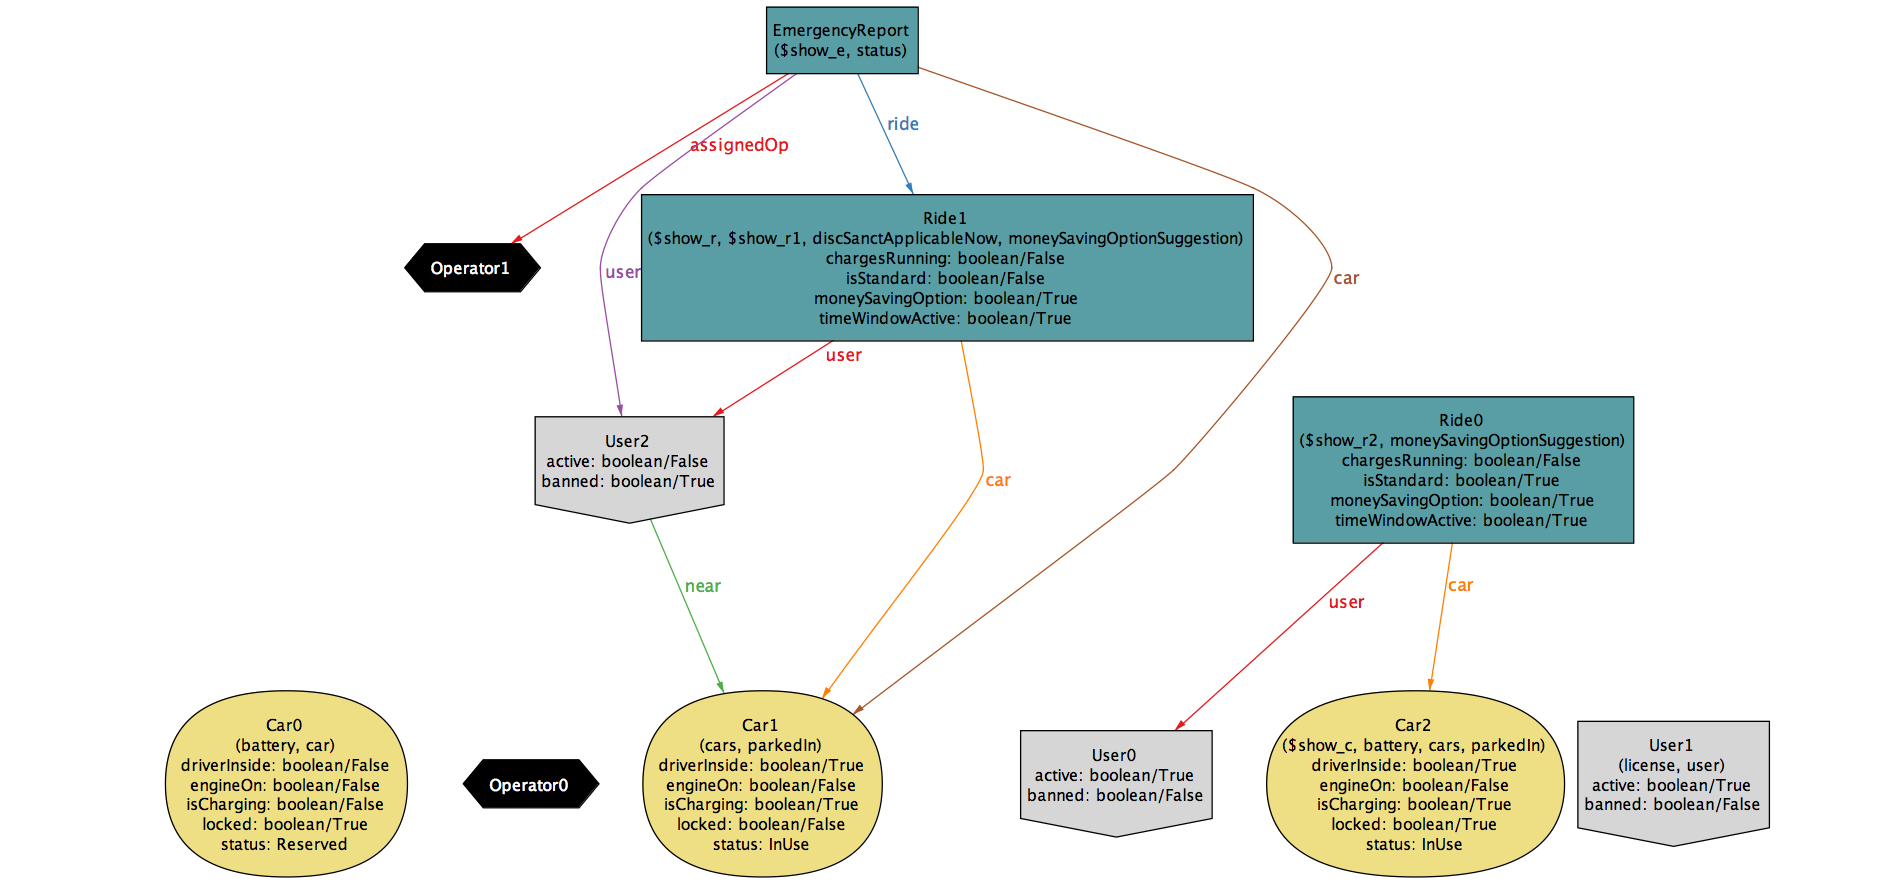
\includegraphics[height=0.9\textheight, center]{img/emergency_reports.png}
	\end{landscape}
